\chapter{Attention}

When a student lacks attention during any class period (or wherever they are when studying/learning), that student is not efficiently learning the material at hand. Without attention, the information cannot be funneled to the brain's learning center. The figure below illustrates the critical role of attention (and motivation) in the learning process.

\begin{marginfigure}%
	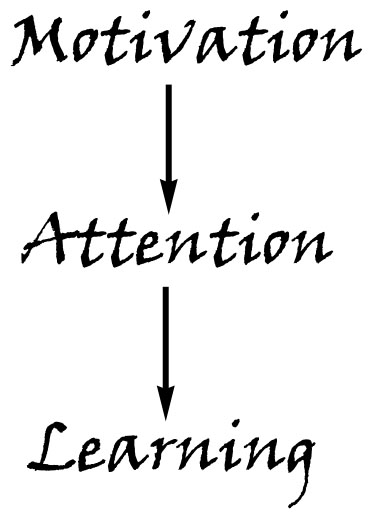
\includegraphics[width=0.75\linewidth]{./images/attention}
	\label{fig:attention}
\end{marginfigure}

This figure starts with motivation. A student must be motivated (intrinsically and/or extrinsically) in order to have attention in class. Motivation is best fueled by an intrinsic source. A student with intrinsic motivation would say ``I like this stuff and its fun to learn''. A student with only extrinsic motivation might say ``This is a required class for me so I'm just doing the minimum so I can graduate''. A student with no motivation would be chatting with a neighbor during class or working a crossword puzzle. Whatever the source, \textbf{motivation leads to attention}. In other words, motivation is a prerequisite to attention. You can't have prolonged attention without motivation. Think of attention as a focus on the material to be learned.

\textbf{Attention leads to learning}. In other words, attention is a prerequisite to learning. And there's no way around it! If a student pays little attention in class, very little learning will occur at that time. I estimate that if a student has good attention in class, it is worth 2-3 hours of study out of class. In other words, \textbf{pay attention in class and it reduces your study time outside of class}.

A student cannot pay attention in class if he/she is sleepy or ill. A good night's sleep will allow the student to be at maximum efficiency  in the classroom. Sleep and health often go together. A lack of sleep makes a person more susceptible to illness. When a student is ill, focus in class is almost impossible. It is also impossible to chat with a neighbor in class and at the same time pay attention to the instructor (or whomever is speaking).

This idea/notion of paying attention in class is one I see many student fail at. I can't tell you how many inattentive students I see each day-it would take too long for me to report.
